\documentclass[11pt,a4paper]{article}
\usepackage[utf8]{inputenc}
\usepackage[T1]{fontenc}
\usepackage[romanian]{babel}
\usepackage[margin=2cm]{geometry}
\usepackage{array}
\usepackage{tabularx}
\usepackage{enumitem}
\setlist{itemsep=2pt,topsep=2pt,parsep=0pt}
\usepackage{graphicx}
\usepackage{setspace}
\usepackage{xcolor}
\usepackage{hyperref}
\usepackage{amssymb}
\setlength{\parindent}{0pt}
\newcommand{\fillline}[1][6cm]{\underline{\hspace{#1}}}
\newcommand{\fillbox}[1][0.4cm]{\framebox[#1]{\rule{0pt}{#1}}}
\newcommand{\checkboxempty}{$\square$}

\begin{document}

\hrule
\vspace{0.15cm}
\noindent
\begin{minipage}[t]{0.40\textwidth}
\vspace{0pt}
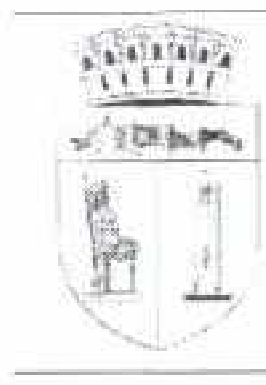
\includegraphics[height=1.5cm]{assets/stema-cluj.png}%
\hspace{0.2cm}%
\raisebox{0.5cm}{\parbox[t]{3.5cm}{\textbf{PRIMĂRIA}\\\textbf{CLUJ-NAPOCA}}}
\end{minipage}%
\begin{minipage}[t]{0.30\textwidth}
\centering
\vspace{0.25cm}

\includegraphics[width=5cm]{assets/barcode-431003.png}
\end{minipage}%
\begin{minipage}[t]{0.30\textwidth}
\raggedleft
\vspace{0.6cm}
Nr. \fillline[3cm] / \fillline[1cm]
\end{minipage}

\vspace{0.3cm}
\hrule
\vspace{0.3cm}

Cerere pentru înscrierea mențiunii de stabilire a domiciliului

\vspace{0.3cm}

\begin{center}
\textbf{Către,}\\
\textbf{PRIMĂRIA CLUJ-NAPOCA}\\
\textbf{Serviciul Public Comunitar Local de Evidență a Persoanelor}
\end{center}

\vspace{0.5cm}

\hspace{1cm}Subsemnatul(a) \underline{ {{nume_complet}} }, CNP \underline{ {{cnp}} },

\vspace{0.3cm}

\hspace{1cm}având domiciliul actual înscris în actul de identitate la adresa:

\vspace{0.2cm}

\underline{ {{adresa_curenta}} }

\vspace{0.3cm}

\hspace{1cm}solicit înscrierea mențiunii de stabilire a domiciliului la noua adresă:

\vspace{0.2cm}

\underline{ {{adresa_noua}} }

\vspace{0.3cm}

\hspace{1cm}Calitatea în care ocup spațiul de locuit de la noua adresă:
\underline{ {{tip_proprietate}} }.

\vspace{0.3cm}

\hspace{1cm}Motivul schimbării domiciliului: \underline{ {{motivul}} }.

\vspace{0.4cm}

\begin{tabularx}{\textwidth}{|X|}
\hline
\textbf{Documente anexate prezentei cereri:}\\
\checkboxempty\ Actul de identitate în original (cu domiciliul actual)\\
\checkboxempty\ Certificate de stare civilă (naștere, căsătorie, copii minori sub 14 ani) --- original\\
\checkboxempty\ Document care atestă dreptul de folosință asupra spațiului de locuit
(act de vânzare-cumpărare / certificat de moștenitor) --- original\\
\checkboxempty\ Extras de carte funciară (emis cu cel mult 30 de zile înainte) --- original\\
\checkboxempty\ Anexa 2 --- declarația găzduitorului, \emph{numai dacă nu sunt proprietarul spațiului}
(alternativ: declarație notarială valabilă 90 de zile sau declarație dată la misiunea diplomatică, valabilă 6 luni)\\
\hline
\end{tabularx}

\vspace{0.4cm}

\hspace{1cm}Declar pe propria răspundere că datele înscrise în prezenta cerere sunt reale și
cunosc că declararea necorespunzătoare a adevărului constituie infracțiune și se pedepsește
conform prevederilor Codului penal.

\vspace{0.3cm}

\hspace{1cm}Am luat la cunoștință că prezența proprietarului spațiului de locuit este
necesară la depunerea cererii și că cererea (Anexa 1) se semnează în fața lucrătorului
de evidență a persoanelor.

\vspace{1cm}

\hspace{1cm}Data \hfill Semnătura\hspace{2cm}

\vspace{0.3cm}

\hspace{1cm}\fillline[3cm] \hfill \fillline[5cm]\hspace{1cm}

\vspace{0.6cm}
\hrule
\vspace{0.3cm}

\begin{center}
\textbf{\footnotesize NU SE COMPLETEAZĂ DE SOLICITANT}
\end{center}

\vspace{0.1cm}

\begin{tabularx}{\textwidth}{|m{4cm}|X|}
\hline
Consimțământul titularului spațiului de locuit & Subsemnatul \fillline[8cm],
posesor al CI/BI seria \fillline[1.5cm] nr. \fillline[3cm], consimt ca solicitantul
prezentei cereri să aibă domiciliul în locuința aflată la adresa înscrisă mai sus.\\
 & Data \fillline[3cm] \hfill Semnătura \fillline[4cm]\\
\hline
Primit cererea și documentele & \fillline[6cm] \hfill \fillline[5cm]\\
 & {\footnotesize (nume și prenume)} \hfill {\footnotesize (semnătura)}\\
\hline
Verificat în evidențe și certific identitatea persoanei & \fillline[6cm] \hfill \fillline[5cm]\\
 & {\footnotesize (nume și prenume)} \hfill {\footnotesize (semnătura)}\\
\hline
\end{tabularx}

\vfill
\hrule
\vspace{0.3cm}

\begin{minipage}[t]{0.65\textwidth}
www.primariaclujnapoca.ro\\
telefon: 0264/596.030\\
Cluj-Napoca, str. Moţilor, nr. 3
\end{minipage}%
\begin{minipage}[t]{0.35\textwidth}
\raggedleft

\includegraphics[width=4cm]{assets/barcode-431003.png}
\end{minipage}

\vspace{0.3cm}
\hrule
\vspace{0.2cm}

{\footnotesize
\textbf{Timp estimativ de completare: 5 minute}

\vspace{0.2cm}

Datele personale care vă sunt solicitate prin prezenta cerere vor fi prelucrate numai în vederea procesării și soluționării solicitării dumneavoastră. Primăria municipiului Cluj-Napoca garantează securitatea procesării datelor și arhivarea acestora în conformitate cu prevederile legale în vigoare.
}

\end{document}
